\documentclass{article}
\usepackage[utf8]{inputenc}
\usepackage[T2A]{fontenc}
\usepackage[english,russian]{babel}
\usepackage{amsmath}
\usepackage{faktor} 
\usepackage{mathrsfs}
\usepackage{amssymb}
\usepackage{mathtools}
\usepackage{amsthm}
\usepackage{float}
\usepackage[shortlabels]{enumitem}
\usepackage[left=2cm,right=2cm, top=2cm,bottom=2cm,bindingoffset=0cm]{geometry}

\DeclareMathOperator{\ord}{ord}
\DeclareMathOperator{\orb}{Orb}
\DeclareMathOperator{\stab}{Stab}
\DeclareMathOperator{\lcm}{lcm}
\DeclareMathOperator{\inn}{Inn}
\DeclareMathOperator{\Ker}{Ker}
\DeclareMathOperator{\im}{Im}
\DeclareMathOperator{\tr}{tr}
\DeclareMathOperator{\rk}{rk}
\DeclareMathOperator{\interior}{int}
\DeclareMathOperator{\conv}{conv}
\DeclareMathOperator{\dom}{dom}
\DeclareMathOperator*{\argmax}{arg\,max}
\DeclareMathOperator{\diag}{diag}
\DeclareMathOperator{\cone}{cone}

\newcommand*{\QED}{\null\nobreak\hfill\ensuremath{\square}}%
\newcommand*{\R}{\mathbb{R}}

\title{Convex functions and Conjugate sets}
\author{Ковалев Алексей}
\date{}

\begin{document}

\maketitle

\section*{Convex functions}
\paragraph{1.} $f(x) = x^d,\, x \in \R_+$
\begin{center}
\begin{tabular}{|c|c|c|c|c|} \hline
    $d$          & выпуклая & вогнутая & строго выпуклая & $\mu$-сильно выпуклая \\ \hline 
    -2           &    да    &    нет   &       да        &          нет         \\ \hline 
    -1           &    да    &    нет   &       да        &          нет         \\ \hline
    0            &    да    &    да    &       нет       &          нет         \\ \hline
    0.5          &    нет   &    да    &       нет       &          нет         \\ \hline
    1            &    да    &    да    &       нет       &          нет         \\ \hline 
    $\in (1; 2)$ &    да    &    нет   &       да        &          нет         \\ \hline
    2            &    да    &    нет   &       да        &      да, $\mu = 2$   \\ \hline
    $> 2$        &    да    &    нет   &       да        &          нет         \\ \hline
\end{tabular}
\end{center}
\begin{itemize}
    \item Проверим на выпуклость: $f''(x) = d(d - 1)x^{d - 2} \geqslant 0 \iff d(d - 1) \geqslant 0 \iff d \in \R \setminus (0; 1)$.
    \item Проверим на вогнутость: $f''(x) = d(d - 1)x^{d - 2} \leqslant 0 \iff d(d - 1) \leqslant 0 \iff d \in [0; 1]$.
    \item Проверим на строгую выпуклость: $f''(x) = d(d - 1) x^{d - 2} > 0 \iff d \in \R \setminus [0; 1]$. 
    \item Проверим на сильную выпуклость: $f''(x) = d(d - 1)x^{d - 2} \geqslant \mu$. Это неравенство не может быть выполнено при $d < 2$, так как при этом $x^{d - 2} \longrightarrow 0$ при $x \longrightarrow \infty$. При $d = 2$ под условие подходит $\mu = 2$. При $d > 2$ неравенство не выполняется, так как в точке $x = 0$ оно имеет вид $0 \geqslant \mu$.
\end{itemize}


\paragraph{2.}
\[ f(x) = -\sum\limits_{k = 1}^n x_k \log x_k, \]
где $\dom f = \{ x \in \R^n_{++} :\: \| x \|_1 = 1 \}$. Ясно, что $\dom f$ -- выпуклое множество. \\
Рассмотрим $g = \sum\limits_{k = 1}^n x_k \log x_k$, определенную на $\R_{++}^n$. Воспользуемся дифференциальным критерием строгой выпуклости 2 порядка.
\[ \nabla^2 g(x) = \diag\left(\frac{1}{x_1},\,\dotsc,\,\frac{1}{x_n}\right) \succ 0, \]
так как $ \forall x \in \R_{++}^n,\, \forall y \in \R^n,\, y \neq 0 \; y^\top \nabla^2 g(x) y = \sum\limits_{k = 1}^n \frac{y_k^2}{x_k} > 0 $. Значит $g$ строго выпукла на $\R_{++}^n$. \\
Если функция строго выпулка на некотором выпуклом множестве $X$, то она строго выпукла и на его выпуклом подмножестве $Y \subset X$. Значит $g$ строго выпукла на $ \dom f $, причем $ -g |_{\dom f} = f $, значит $f$ строго вогнута на $\dom f$. \QED
% \begin{equation*}
% \begin{aligned}
%     -f(\lambda x &+ (1 - \lambda) y) + \lambda f(x) + (1 - \lambda) f(y) \\
%     &= \sum\limits_{i = 1}^n (\lambda x_i + (1 - \lambda) y_i) \log (\lambda x_i + (1 - \lambda) y_i) - \lambda \sum_{i = 1}^n x_i \log x_i - (1 - \lambda) \sum_{i = 1}^n y_i \log y_i \\
%     &= \lambda \sum_{i = 1}^n x_i \log \frac{\lambda x_i + (1 - \lambda) y_i}{x_i} + (1 - \lambda) \sum_{i = 1}^n y_i \log \frac{\lambda x_i + (1 - \lambda) y_i}{y_i}
% \end{aligned}
% \end{equation*}
% Рассмотрим эту сумму при каком-то конкретном $i$, предположив, не умаляя общности, что $y_i < x_i$.
% \begin{equation*}
% \begin{aligned}
%     \lambda x_i \log \frac{\lambda x_i + (1 - \lambda) y_i}{x_i} &+ (1 - \lambda) y_i \log \frac{\lambda x_i + (1 - \lambda) y_i}{y_i} \\
%     &< \lambda x_i \log \frac{\lambda x_i + (1 - \lambda) y_i}{x_i} + (1 - \lambda) x_i \log \frac{\lambda x_i + (1 - \lambda) y_i}{y_i} \\
%     &= \lambda x_i \log \frac{y_i}{x_i} + x_i \log \frac{\lambda x_i + (1 - \lambda) y_i}{y_i} \\
%     &= x_i \log \left( \frac{y_i^\lambda}{x_i^\lambda} \cdot \frac{\lambda x_i + (1 - \lambda) y_i}{y_i} \right) \\
%     &= x_i \log \frac{\lambda x_i + (1 - \lambda) y_i}{x_i^\lambda y_i^{1 - \lambda}} \\
% \end{aligned}
% \end{equation*}
% Причем $\log \frac{\lambda x_i + (1 - \lambda) y_i}{x_i^\lambda y_i^{1 - \lambda}} < 0 \iff \lambda x_i + (1 - \lambda) y_i < x_i^\lambda y_i^{1 - \lambda} $.


\paragraph{3.} $ f:\: \R_{++}^n \to \R,\, f(x) = - \prod\limits_{i = 1}^n x_i^{\alpha_i},\, \mathbf{1}^\top \alpha = 1,\, \alpha \succeq 0 $. \\
To be done...


\paragraph{4.} $ P = \conv\{ v_1,\, v_2\, \dotsc,\, v_k \},\, f :\: P \to \R$ -- выпуклая. \\
Для любой точки $ x = \sum\limits_{n = 1}^k \theta_n v_n \in P$, где $\sum\limits_{n = 1}^k \theta_n = 1,\, \theta_n \geqslant 0$ выполняется неравенство Йенсена (в таком виде его можно получить применив $k - 1$ раз определение выпуклой функции), то есть
\[ f\left( \sum_{n = 1}^k \theta_n v_n \right) \leqslant \sum_{n = 1}^k \theta_n f(v_n) \]
Пусть $\argmax\limits_{n = 1,\,\dotsc,\,k} f(v_n) = i$, то есть среди $v_n$ максимум достигается на вершине $v_i$ (возможно и на других, в таком случае выберем одну произвольную). Тогда 
\[ f\left( \sum_{n = 1}^k \theta_n v_n \right) \leqslant \sum_{n = 1}^k \theta_n f(v_n) \leqslant \sum_{n = 1}^k \theta_n f(v_i) = f(v_i) \]
Иными словами $ \sup\limits_{x \in P} f(x) \leqslant f(v_i) $, причем очевидно, что на $v_i$ он достигается. Значит $ \sup\limits_{x \in P} f(x) = \max\limits_{n = 1,\,\dotsc,\,k} f(v_k) $. \QED 


\paragraph{5.}
\begin{enumerate}[(a)]
    \item $f$ является $\mu$-сильно выпуклой $\iff$ $ \exists \mu > 0 :\: \forall x_1,\, x_2 \in S,\, \forall \lambda \in [0; 1] $ 
        \[ f(\lambda x_1 + (1 - \lambda) x_2) \leqslant \lambda f(x_1) + (1 - \lambda) f(x_2) - \mu\lambda(1 - \lambda) \| x_1 - x_2 \|^2 \]
    \item $f$ является $\mu$-сильно выпуклой $\iff$ $ \exists \mu > 0 :\: f(x) - \mu\|x\|^2 $ является выпуклой.
\end{enumerate}
% Покажем сначала (a) $\Longrightarrow$ (b):
% \[ f(\lambda x_1 + (1 - \lambda) x_2) \leqslant \lambda f(x_1) + (1 - \lambda) f(x_2) - \mu\lambda(1 - \lambda) \| x_1 - x_2 \|^2 \]
% \begin{equation*}
% \begin{aligned}
%     f(\lambda x_1 + (1 - \lambda) x_2) &- \lambda f(x_1) - (1 - \lambda) f(x_2) \\
%     &\leqslant -\mu \lambda (1 - \lambda) \|x_1 - x_2\|^2 \\
%     &\leqslant -\mu \lambda (1 - \lambda) \left( \|x_1\|^2 + \|x_2\|^2 - 2 \|x_1\| \cdot \|x_2\| \right) \\
%     &\leqslant \mu \left( \lambda^2 \|x_1\|^2 + (1 - \lambda)^2 \|x_2\|^2 + 2 \lambda (1 - \lambda) \|x_1\| \cdot \|x_2\| - \lambda \|x_1\|^2 - (1 - \lambda) \|x_2\|^2 \right) \\
%     &\leqslant \left( \mu \| \lambda x_1 + (1 - \lambda) x_2 \|^2 - \mu \lambda \|x_1\|^2 - \mu (1 - \lambda) \|x_2\|^2 \right) \\
% \end{aligned}
% \end{equation*}
% \[ f(\lambda x_1 + (1 - \lambda) x_2) - \frac12 \tilde\mu \| \lambda x_1 + (1 - \lambda) x_2 \|^2 \leqslant \lambda f(x_1) + (1 - \lambda) f(x_2) - \frac12 \tilde\mu \lambda \|x_1\|^2 - \frac12 \tilde\mu (1 - \lambda) \|x_2\|^2 \]
% Значит $f(x) - \frac12 \tilde\mu \|x\|^2$ -- выпуклая. \\
% Теперь в другую сторону (b) $\Longrightarrow$ (a):
To be done...


\section*{Conjugate sets}
\paragraph{1.} $ \mathbb{A}_n = \{ A:\: A \in \R^{n \times n},\, A^\top = -A \} $.
\begin{itemize}
    \item Пусть $ X \in \mathbb{A}_n^\ast $. Тогда $ \forall A \in \mathbb{A}_n \; \langle A,\, X \rangle \geqslant 1 $. То есть $ \langle A,\, X \rangle \tr A^\top X = -\tr AX \geqslant -1 $. Рассмотрим $A$, такую что $A_{ij} = q,\, A_{ji} = -q$, а все остальные элементы -- нули. Тогда $ \tr AX = q X_{ji} - q X_{ij} \leqslant 1 $. То есть при $q > 0$ имеем $ X_{ji} \leqslant X_{ij} + \frac{1}{|q|} $, а при $q < 0$ имеем $X_{ji} \geqslant X_{ij} - \frac{1}{|q|}$. В силу произвольности $q$ это значит, что $X_{ij} = X_{ji}$. Значит $ \mathbb{A}_n^\ast \subset \mathbb{S}_n $.
    \item Пусть $ X \in \mathbb{S}_n,\, A \in \mathbb{A}_n $. $\mathbb{A}_n $ образует линейное пространство с базисом из матриц $E_{ij},\, i \neq j$, где $E_{ij} = -E_{ji} = 1$. Тогда $ \langle A,\, X \rangle = \tr A^{\top}X = -\tr AX = \sum\limits_{1 \leqslant i < j \leqslant n} q_{ij} \tr E_{ij} X = \sum\limits_{1 \leqslant i < j \leqslant n} q_{ij} (X_{ji} - X_{ij}) = 0 \geqslant -1 $. 
\end{itemize}
Значит $\mathbb{A}_n^\ast = \mathbb{S}_n$. \QED


\paragraph{2.} $ S = \left\{ x \in \R^2 :\: x_1 + x_2 \geqslant 0,\, -\frac12 x_1 + x_2 \geqslant 0,\, 2x_1 + x_2 \geqslant - 1,\, -2x_1 + x_2 \geqslant -3 \right\}. $ \\
Ясно, что $S$ -- замкнутое множество, выпуклое множество (как надграфик выпуклой функции, полученной как максимум линейныx), $0 \in S$. Значит $S^{\ast\ast} = \overline{\conv(S \cup \{0\})} = S$. Так как $S^\ast$ всегда замкнуто и содержит 0, то $S^{\ast\ast\ast} = S^\ast$. Остается лишь найти само $S^\ast$. \\
Представим $S$ в виде $S = \conv\!\big((0,\, 0),\, (-1,\, 1),\, (2,\, 1)\big) + \cone\!\big( (1,\, 2),\, (-1,\, 2) \big)$. Это абсолютно очевидно геометрически, но можно показать и непосредственно (но я этого делать не буду, потому что лень).
Тогда согласно теореме о сопряженном к многограннику множеству 
\[ S^\ast = \{ p \in \R^2 :\: -p_1 + p_2 \geqslant - 1,\, 2 p_1 + p_2 \geqslant - 1,\, p_1 + 2 p_2 \geqslant 0,\, -p_1 + 2 p_2 \geqslant 0 \}. \]
\begin{figure}[H]
    \centering
    \begin{minipage}[b]{0.45\textwidth}
        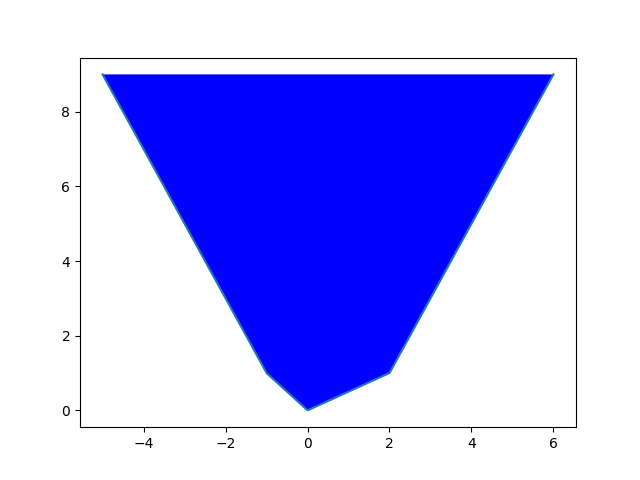
\includegraphics[scale=0.5]{plot.png}
        \caption{Множество $S$}
    \end{minipage}
    \begin{minipage}[b]{0.45\textwidth}
        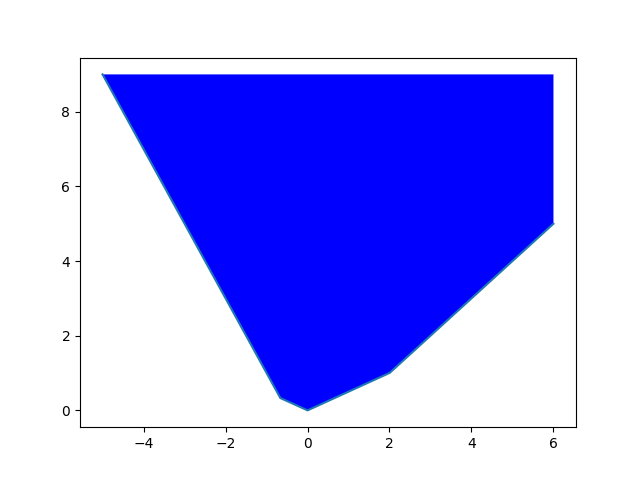
\includegraphics[scale=0.5]{plot_.png}
        \caption{Множество $S^\ast$}
    \end{minipage}
\end{figure}


\paragraph{3.} $ B_p = \{ x \in \R^n :\: \|x\|_p \leqslant 1 \},\, \frac{1}{p^\ast} + \frac{1}{p} = 1. $ \\
В любой норме единичный шар является замкнутым, выпуклым и содержит 0, значит $B_p^{\ast\ast} = B_p$. Тогда если $B_{p^\ast} = B_p^\ast$, то и $B_{p^\ast}^\ast = B_p^{\ast\ast} = B_p$.
\begin{itemize}
    \item Пусть $y \in B_{p^\ast},\, x \in B_p$. Воспользуемся неравенство Гельдера
    \[ \left| \langle x,\, y \rangle \right| = \left| \sum_{k = 1}^n x_k y_k \right| \leqslant \sum_{k = 1}^n | x_k y_k | \leqslant \|x\|_p \|y\|_{p^\ast} \leqslant 1. \]
    Значит $ \langle x,\, y \rangle \geqslant -1,\, y \in B_p^\ast$ и $ B_{p^\ast} \subset B_p^\ast $. 
    \item To be done...
\end{itemize}


\end{document}
